\documentclass[10pt,twocolumn,letterpaper]{article}

\usepackage{cvpr}
\usepackage{times}
\usepackage{epsfig}
\usepackage{graphicx}
\usepackage{amsmath}
\usepackage{amssymb}
\usepackage{float}

% Include other packages here, before hyperref.

% If you comment hyperref and then uncomment it, you should delete
% egpaper.aux before re-running latex.  (Or just hit 'q' on the first latex
% run, let it finish, and you should be clear).
\usepackage[pagebackref=true,breaklinks=true,letterpaper=true,colorlinks,bookmarks=false]{hyperref}

\cvprfinalcopy % *** Uncomment this line for the final submission

\def\cvprPaperID{****} % *** Enter the CVPR Paper ID here
\def\httilde{\mbox{\tt\raisebox{-.5ex}{\symbol{126}}}}

% Pages are numbered in submission mode, and unnumbered in camera-ready
\ifcvprfinal\pagestyle{empty}\fi
\begin{document}

%%%%%%%%% TITLE
\title{Unsupervised Character Recognition in Cartoons}

\author{Nishad Mudras \\
{\tt\small nmudras@cs.umass.edu}
% For a paper whose authors are all at the same institution,
% omit the following lines up until the closing ``}''.
% Additional authors and addresses can be added with ``\and'',
% just like the second author.
% To save space, use either the email address or home page, not both
\and
Prateek Sharma \\
{\tt\small prateeks@cs.umass.edu}
}

\maketitle
%\thispagestyle{empty}

%%%%%%%%% ABSTRACT
\begin{abstract}
  In this project we present the design and implementation, and evaluate
an unsupervised system for recognition of the \emph{main character} of
an animated cartoon video. The main character (not to be confused with a
text character!)is the person who occurs in the largest number of
scenes in a video. Our approach eschews the commonly found
supervised-learning based techniques, and instead is \emph{completely
  unsupervised}.

\end{abstract}

%%%%%%%%% BODY TEXT
\section{Introduction}
In this project we present the design and implementation, and evaluate
an unsupervised system for recognition of the \emph{main character} of
an animated cartoon video. The main character (not to be confused with a
text character!)is the person who occurs in the largest number of
scenes in a video. Our approach eschews the commonly found
supervised-learning based techniques, and instead is \emph{completely
  unsupervised}.


\subsection{Unsupervised Learning}

An unsupervised approach does not require labelled training data, a
situation which is predominant because of the difficulties in
acquiring high quality human-labelled training sets. While
human-curated labelled data exist for a significant fraction of
computer vision tasks (for example the SIFT descriptors), they are not
universally available. The goal of this project was to explore and
evaluate how far the unsupervised learning approach can be pushed in
the character recognition domain.

On the flip-side, unsupervised learning also has many disadvantages,
as we quickly learned. The lack of ground-truth presents a
particularly nasty challenge. Without 

\subsection{Why Cartoons}
This project focuses on recognizing characters in cartoons. Using
cartoons as the environment in which we perform the recognition task
has several important advantages which are manifested due to their
simplistic visual nature.

Cartoons (see Figure~\ref{sample-cartoons} for a few example frames)
have a relatively simple visual style. Textures are mostly
non-existent, and colors are either solidly filled or simple gradients
are used. The edges in the images are also smooth, with well defined
curves. All of these features are artifacts of the cartoon creation
process. While more modern cartoons may have a sophisticated visual
style, we focus our attention to the simpler styles which are found in
the vast majority.


\subsection{Scope of this project}
We study unsupervised techniques in cartoon character recognition. Our
dataset consists of \emph{SouthPark} videos, a popular
animated-cartoon TV series. While it was our intent to explore the
application of our technique to several other animated cartoons as
well (for example \emph{Simpsons, Family Guy, Pokemon}), we decided to
restrain our focus to only SouthPark. 

Given a video, our end-goal is to provide the list of scenes(or
frames) in which any character appears. Alternatively, this can also
be thought about as identifying characters in a given frame. Using
this \emph{appearance information}, we can provide analysis to answer
questions such as:

\begin{itemize}
\item Which scenes does a character occur?
\item Who is the main character in this video? The main character is
  the one who occurs in the largest number of scenes
\item What is the percentage of scenes in which a character occurs?
  This can be used to improve the information retrieval in videos by
  providing an additional query parameter. For example, users might
  want to search for videos in which their favourite character occurs
  in atleast 50\% of the scenes etc.
\end{itemize}

\section{Background and Related Work}

In order to detect people, the standard approach is to use a face
recognition technique, since face recognition is a well understood
problem. Because it relies on human face structure, face detection
algorithms do no work with cartoon images at all because of the
``cartoonish'' nature of the faces with exaggerated features etc. As a
result, one of the primary techniques for character recognition is
ruled out. 

Character detection in video sequences is a fairly well studied
problem~\cite{everingham2009taking,
  satoh1999name,snoek2008concept,sivic2005person}. Most of the work
~\cite{arandjelovic2005automatic} relies on face recognition, since
human face recognition is a well studied problem as well. As noted
earlier, face detection/recognition does not work for animated
cartoons, and thus a vast majority of literature in this area is of
little use to us.

For the animated cartoon domain, the results are not as
numerous. \cite{zhang20132} uses multi-scale shape detection and a
supervised machine learning approach, which is in contrast to our
unsupervised approach.



\section{Design}
As mentioned previously, the focus of our design has been the use of
unsupervised techniques. This section outlines the design of our image
processing pipeline. We describe the high-level idea, the techniques
used, and the alternatives to some the design decisions we took.

\subsection{High-level pipeline}
We assume that the entire video for which the character detection
needs to be performed is given as the input. The pipeline makes 2
passes over the video, and thus a streaming approach would not
work. We discuss an alternate solution which can work in the streaming
setting later.

Below is the high-level pipeline, with each step explained in detail
later:
\begin{enumerate}
\item Input: A video file
\item Process the video to extract frames. A sampling of frames is
  done to extract 2 frames per second instead of 24.
\item Scene detection. Even after the frame sampling, the changes in
  frames is small. We identify scene changes and pick a representative
  frame for a scene. All the rest of the frames are discarded. 
\item For each frame, we perform segmentation and extract the image segments.
\item Each segment is processed to produce the features.
\item All the segments(and their features) from all the frames are
  then clustered to form a dictionary of segments.
\item Clusters which represent a whole or part of the characters are identified
\item The scene frames are processed again. They may be resegmented
  again, and we assign each segment 
\end{enumerate}

\subsection{Scene detection}
To detect changes in scenes, we inspect changes between consecutive
frames. The frames are subtracted to form a \emph{diff frame}. If the
pixels dont change between frames, the diff frame is all zeroes. Any
non-zeroes are indicative of a change. If the changes are above a
certain threshold, the scene has changed. A small threshold yields a
larger number of scenes, whereas a larger threshold is more sensitive
to scene changes. 

Using the scene detection, we are able to extract about 200 frames
from a 20 minute episode. 

\subsection{Segmentation}

Once frames from the video have been sampled (by using scene detection
above), we process each frame independently to extract the
\emph{segments} from the image. 

A crucial assumption/hypothesis of our project has been that
\emph{segments are good proxies for objects in animated cartoons}.  We
have evaluated this hypothesis for a large variety of segmentation
algorithms (see Figure ~\ref{diff-segmentations}). Visual inspection
(since we do not posses ground truth data) strongly suggests that
objects (such as the characters' headgear, faces, clothes etc) are
easily segmented from most frames. Ofcourse, we as yet do not know
which segment corresponds to which object, which is considered in the
next step. 

\begin{figure*}[ht]
  \centering
  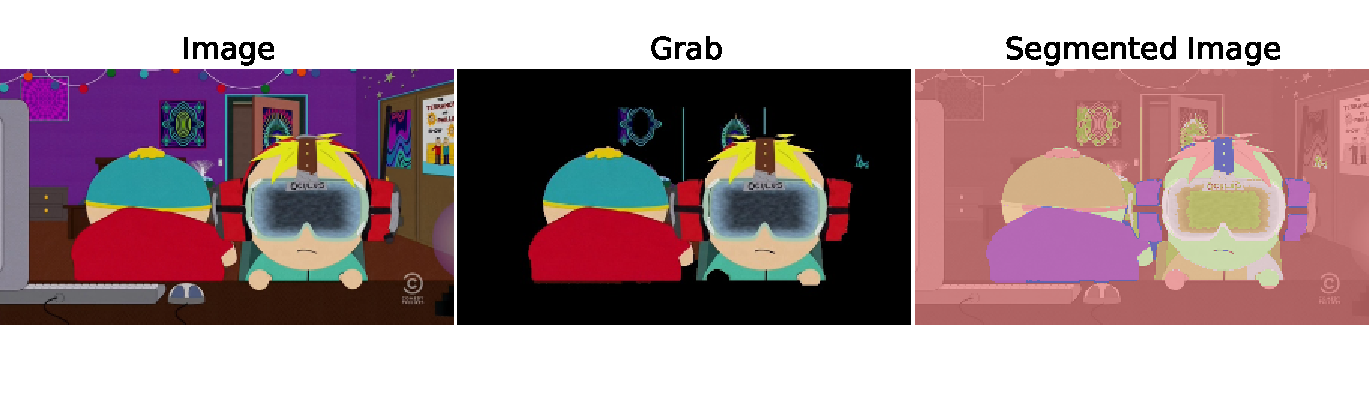
\includegraphics[width=0.9\textwidth]{../seg2.pdf}
  \caption{The result of the segmentation step of the
    pipeline. Grabcut is able to remove the background, and the
    norm-cut segmentation algorithm yields the segments}
  \label{diff-segmentations}
\end{figure*}

We have the evaluated the effectiveness of Normalized-cuts, Watershed
and QuickShift with different choice of parameters. Because its
difficult to show the effectiveness of these without ground-truth, we
do not include the results of the segmentation process, since a lot of
it was done by visual inspection on a large number of frames to
determine effectiveness.  Both Watershed and normalized-cuts worked
equally well, but use normalized-cuts as our primary segmentation
algorithm because of the lack of any pre-processing (as required by
watershed) and also because the number of segments can be given as a
parameter to the normalized-cut algorithm. 

The question then is how to determine the number of segments. Certain
frames have a lot more segments than others. To solve this problem, we
use the Grab-cut technique to extract the foreground of every
frame. This eliminates the background noise in the images , and
provides a filtered image for the segmentation algorithm. Grabcut
requires a bounding box as the input. We provide the entire frame
(minus a small border strip) to Grab-cut. Figure ~\ref{grabcut} shows
the results of grabcut being applied on some frames. We can see that
the background is removed from the images quite nicely. After grabcut,
the maximum number of segments we segment the image into is
\emph{20}. If fewer number of segments are detected, then norm-cut
outputs fewer segments. Too few segments clusters multiple objects
into one. Whereas a larger number of segments will break down an
object into many segments. A ``perfect'' segmentation for us yields a
one-to-one correspondence between objects and segments (an entire
object is represented as one segment). 

\begin{figure}[H]
  \centering
  
\includegraphics[width=0.5\textwidth]{../results/southpark.png}
  \caption{Original Image}
  \label{orig-image}
\end{figure}


\begin{figure}[H]
  \centering
  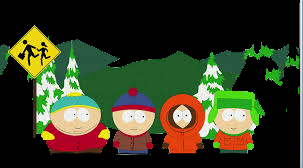
\includegraphics[width=0.5\textwidth]{../results/grabcut_full.png}
  \caption{Grabcut effectiveness}
  \label{grabcut}
\end{figure}

\subsection{Feature extraction}
Each segment is processed independently to extract features from
it. For animated cartoons the features that work best for animated
cartoons are:
\begin{enumerate}
\item \textbf{The color of the segment. } We've observed that most
  segments are of predominantly one color. Thus, the average color
  across all the pixels of a segment can work as a feature. Another
  approach is to cluster the colors into a small number of colors (say
  3) and use the cluster centres as features. The cluster centres are
  also weighted by their frequency (histogram).  The intuition for
  using color as a feature is to detect clothing of characters, since
  characters mostly wear the same clothes. Thus the cap, jacket are
  segmented into their own segments, and are of uniform color
  throughout for a large number of scenes.

\item \textbf{Segment shape. } We can also use the segment
  \emph{shape} as the a feature. We use the HOG features, and apply on
  each segment. This seems like an appealing at first, but does not
  seem very useful in increasing the accuracy of
  classification. Object shape has two problems. First, objects
  belonging to different characters are similarly shaped. The
  head,faces,jackets are all very similarly shaped. Thus we dont get
  specificity. Second, due to changing perspectives and angles, the
  shape does not remain constant over scenes either. 

\end{enumerate}

\subsection{Dictionary creation using clustering} 

Once all the features from the images have been extracted, we store
them for later use. The features are then fed to a clustering
algorithm such as k-means. We have use 3 different clustering
algorithms: kmeans, Agglomerative clustering, and DBSCAN. These are
evaluated in the next section(Evaluation).

The choice for the number of clusters is a very important one. While
silhoutte scores guided us to use higher values for the number of
clusters, having too many clusters makes the job of recognition more
difficult. This is the key tradeoff. If there are too many clusters,
then the association rules (cluster $c$ maps to object $d$) become
much harder, since we lose the bijective property and need multiple
clusters to represent the same object.

On the other hand, having fewer number of clusters means that the
clusters are shared between objects. This is an even worse problem,
since now we need to resort to other techniques. Accordingly, we have
set the number of clusters in the 150-300 range.


\subsection{HSV color representation for clustering}



Specifically for cartoons, it was hypothesized that use of the HSV
color space for clustering using k-means, instead of the RGB
representation, would provide more tightly bound and accurate
clusters.  This was due to the fact that in cartoons, for a given
object color (shirt, hat, etc.), the hue value remains almost same
across multiple frames, while the saturation and value components
might show few changes depending on the time of the day in a
particular scene. As opposed to this, RGB can show variations across
all its three components based on variations in light, which can skew
the distance-based clustering process of k-means. The HSV color space
enables the separation of the chrominance information from the
luminance information, thus providing components such as color,
vibrancy and brightness, as opposed to the RGB color space that
doesn’t provide a distinction between these factors.

\begin{figure*}[H]
  \centering
  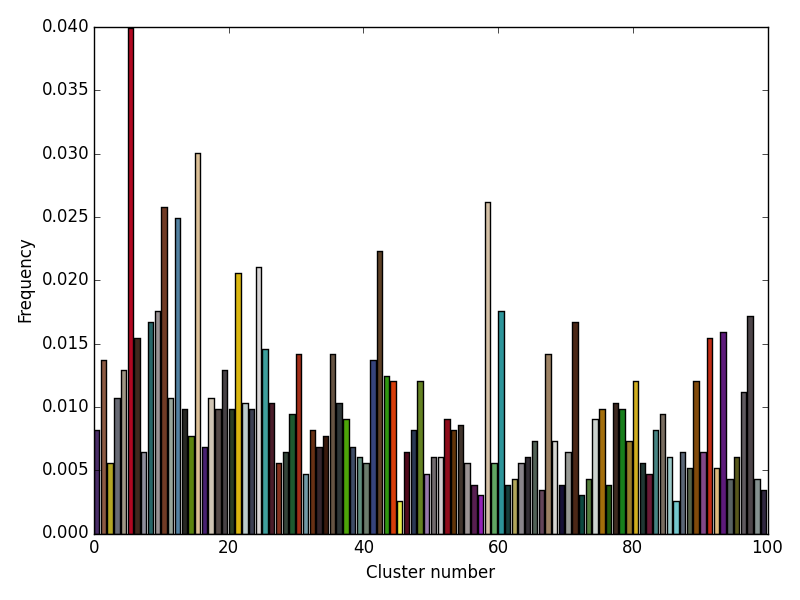
\includegraphics[width=0.9\textwidth]{hsv.png}
  \caption{K-means histogram with the HSV feature vectors}
  \label{hsv}
\end{figure*}

\begin{figure*}[H]
  \centering
  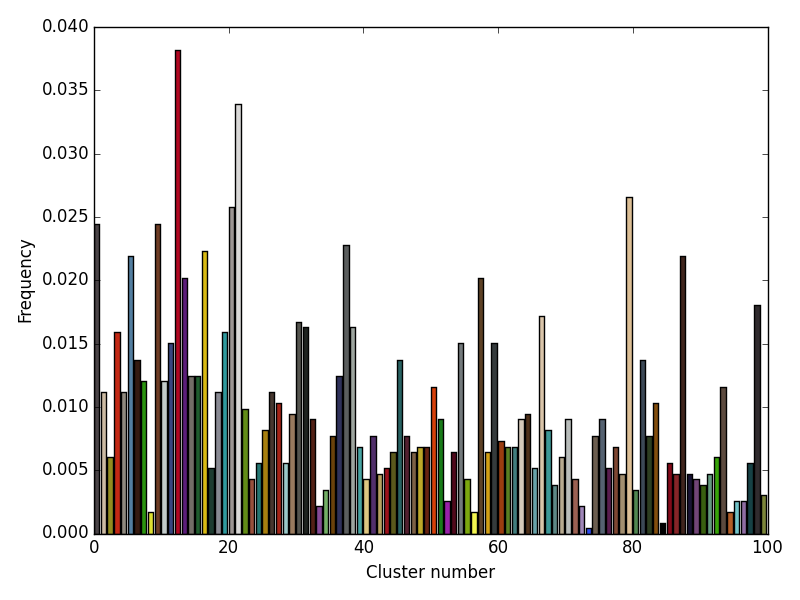
\includegraphics[width=0.9\textwidth]{rgb.png}
  \caption{K-means histogram with the RGB feature vectors}
  \label{rgb}
\end{figure*}



As seen in Figures~\ref{hsv,rgb}, the difference between the largest
of clusters’ sizes is more pronounced in results using HSV than using
RGB. Also, the secondary cluster (i.e. the second largest cluster)
represents the skin, which is as desired, since the component occurs
across almost all the frames - while such a cluster in RGB
representation is skewed; an unrecognizable color is obtained, which
could be resultant of different colored segments clustered together.

\subsection{Segment recognition}

Once we have obtained a dictionary, the next step is to actually
recognize the objects. We again grabcut and segment the image to
obtain the segments, and get the feature vectors for each segment. The
problem now is to assign segments to cluster centres.

A straightforward approach is to simply assign segments to their
closest cluster-centre, a step supported by all the clustering
algorithm implementations. This is a ``greedy'', local way of
assigning \emph{labels} to the segments. A more sophisticated strategy
that we have tried is to instead consider pairs of neighbouring
segments, and then do find a pair of clusters which minimize the
distance to both the corresponding segments. 

The problem now is : \emph{How to recongnize objects from labels?}.
Again, availability of ground-truth or tagged data would prove
immensely useful here. An automated way of assigning labels(clusters)
to objects is to use a frequency count of the labels in the clustering
histogram.. If a label occurs very often, it is likely to belong to
the leading characters of the episode since they occur in a larger
majority of the scenes . An advantage of this method is that this is
completely automated, and also robust to changes in style and between
episodes , and can work equally well for all the episodes because we
use a per-episode dictionary. This approach can also be used with a
global multi-episode dictionary, wherein we train on a few episodes,
create the dictionary, and then use this single dictionary on
other(new, unprocessed) episodes.

But there are many characters, so how do we determine their
``correct'' labels?  This is where we use an auxiliary authoritative
dictionary. That is, we obtain a few ``canonical'' images for each
character. Then, we do the segmentation and clustering on these
canonical images, to identify the actual label of the segments. (Note
that in our case, segments are proxies for objects). Thus, we now have
a ``gold-standard'' mini-dictionary, using which we identify the
clusters in the actual complete dictionary (obtained earlier by kmeans
above). This gives us association rules like:

\begin{itemize}
\item If label==2 Then segment is Cartman's Hat
\item If label==2 or label==3 Then segment is Cartman's jacket
\item If label==2 and neighbouring label==5 Then ...
\end{itemize}

\subsection{Character recognition}

Now that we have recognized the segments, we need to combine them into
actual characters, since a character can be composed of multiple
segments, we use a simple agglomerative rules. These rules are of the
form:

\begin{itemize}
\item If Cartman's hat is detected , then cartman exists in the scene
\end{itemize}

Obviously, if multiple objects are detected, that increases the
confidence of our prediction. We ensure two objects are detected
before concluding that the character exists in the frame.

\section{Implementation}
The pipeline is implemented by using the \texttt{scikit-image} and
\texttt{opencv} libraries. For clustering, the \texttt{scikit-learn}
toolkit was utilized.



\section{Evaluation}

The primary difficulty in evaluation was the lack of ground-truth data
at every step of the pipeline. As a result, most of the evaluation was
done manually by ``eye-balling'' the output at each step and then
trying to understand the results.


\begin{table}
\begin{tabular}{|l|c|}
  \hline
  Parameter & Value \\
  \hline
Number of scenes extracted from one episode & 300  \\

Segments per image & 10 \\

Feature vector length &  3  \\
  
  \hline
\end{tabular}
\caption{Average numbers for the experiments}
\end{table}


\subsection{Segmentation Analysis}

\subsection{Clustering Histograms}

\begin{figure}[p]
  \centering
  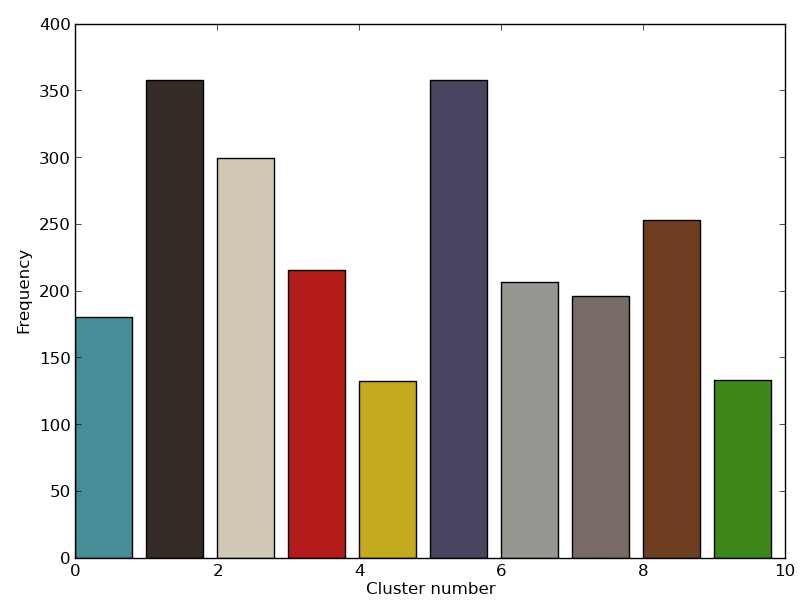
\includegraphics[width=0.50\textwidth]{../results/10_histogram.png}
  \caption{kmeans histogram with k=10}
  \label{k-10}
\end{figure}

\begin{figure}[p]
  \centering
  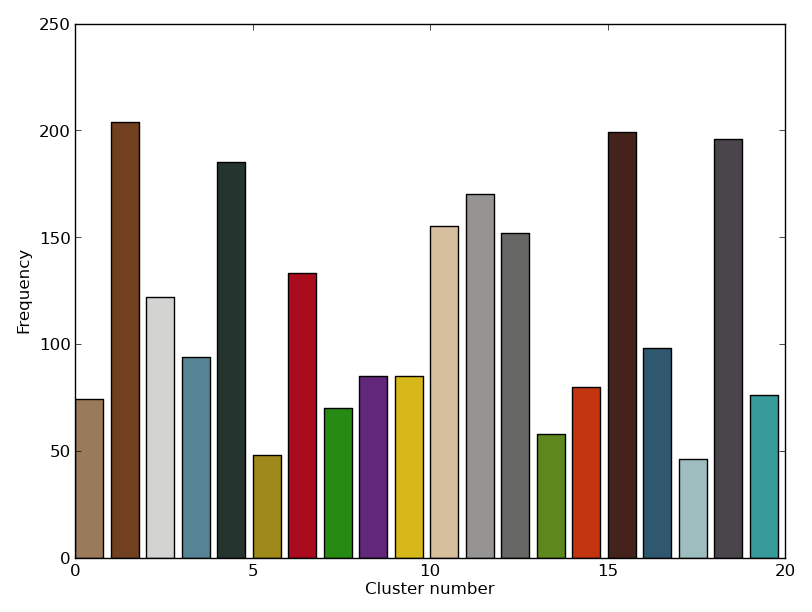
\includegraphics[width=0.50\textwidth]{../results/20_histogram.png}
  \caption{kmeans histogram with k=20}
  \label{k-20}
\end{figure}

\begin{figure}[p]
  \centering
  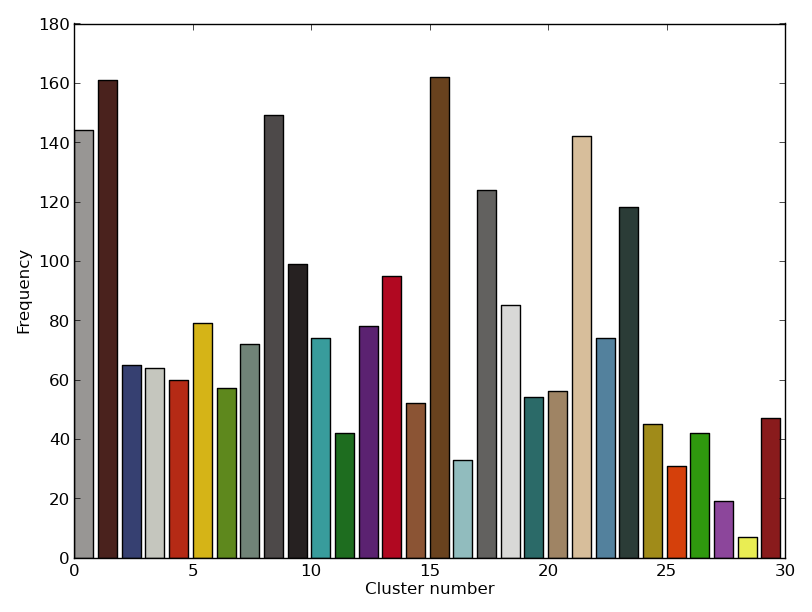
\includegraphics[width=0.50\textwidth]{../results/30_histogram.png}
  \caption{kmeans histogram with k=30}
  \label{k-30}
\end{figure}

\begin{figure*}[p]
  \centering
  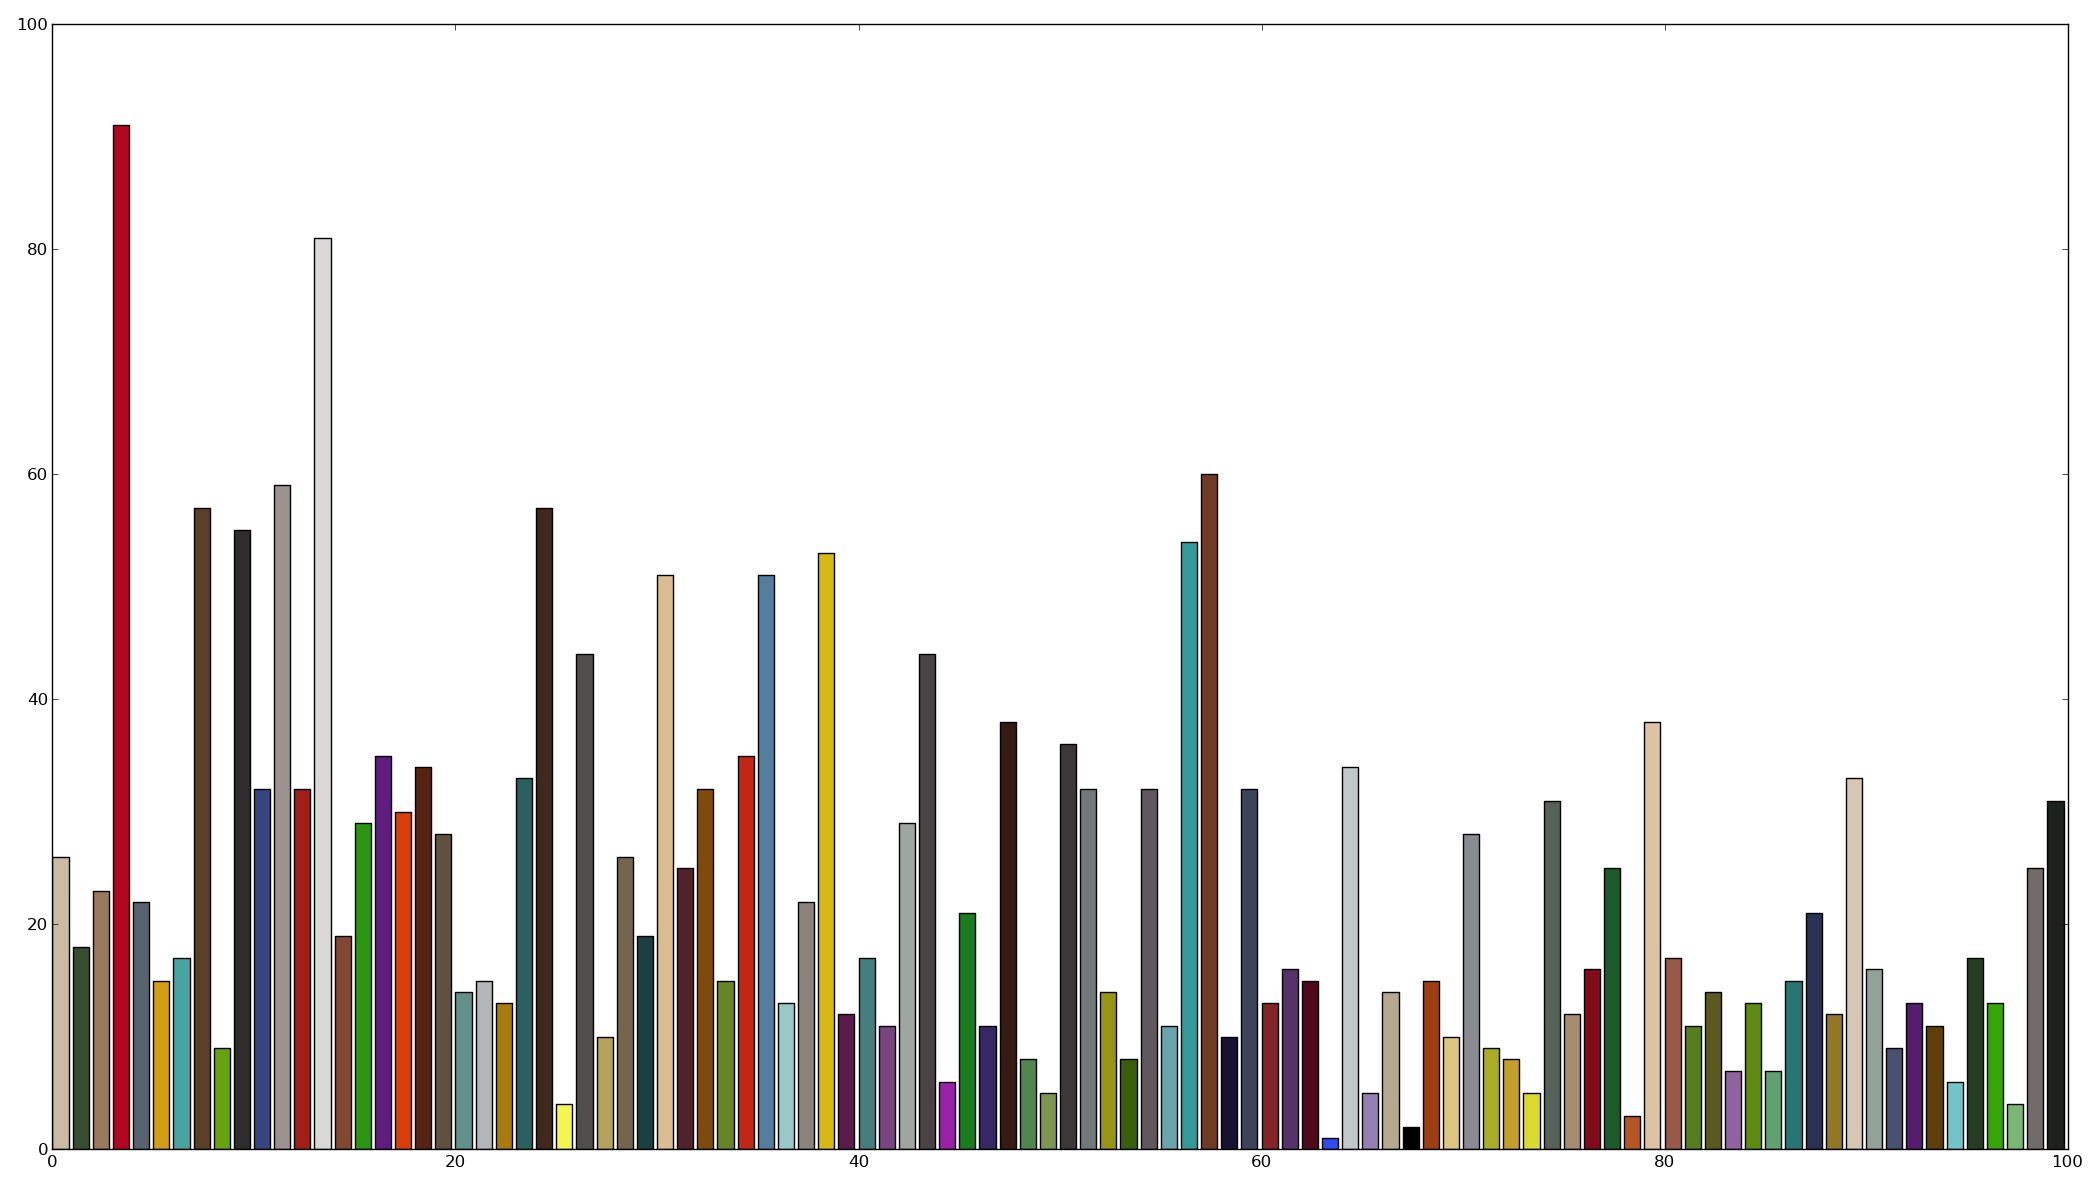
\includegraphics[width=0.90\textwidth]{../results/100_histogram.png}
  \caption{kmeans histogram with k=100}
  \label{k-30}
\end{figure*}

\begin{figure*}[p]
  \centering
  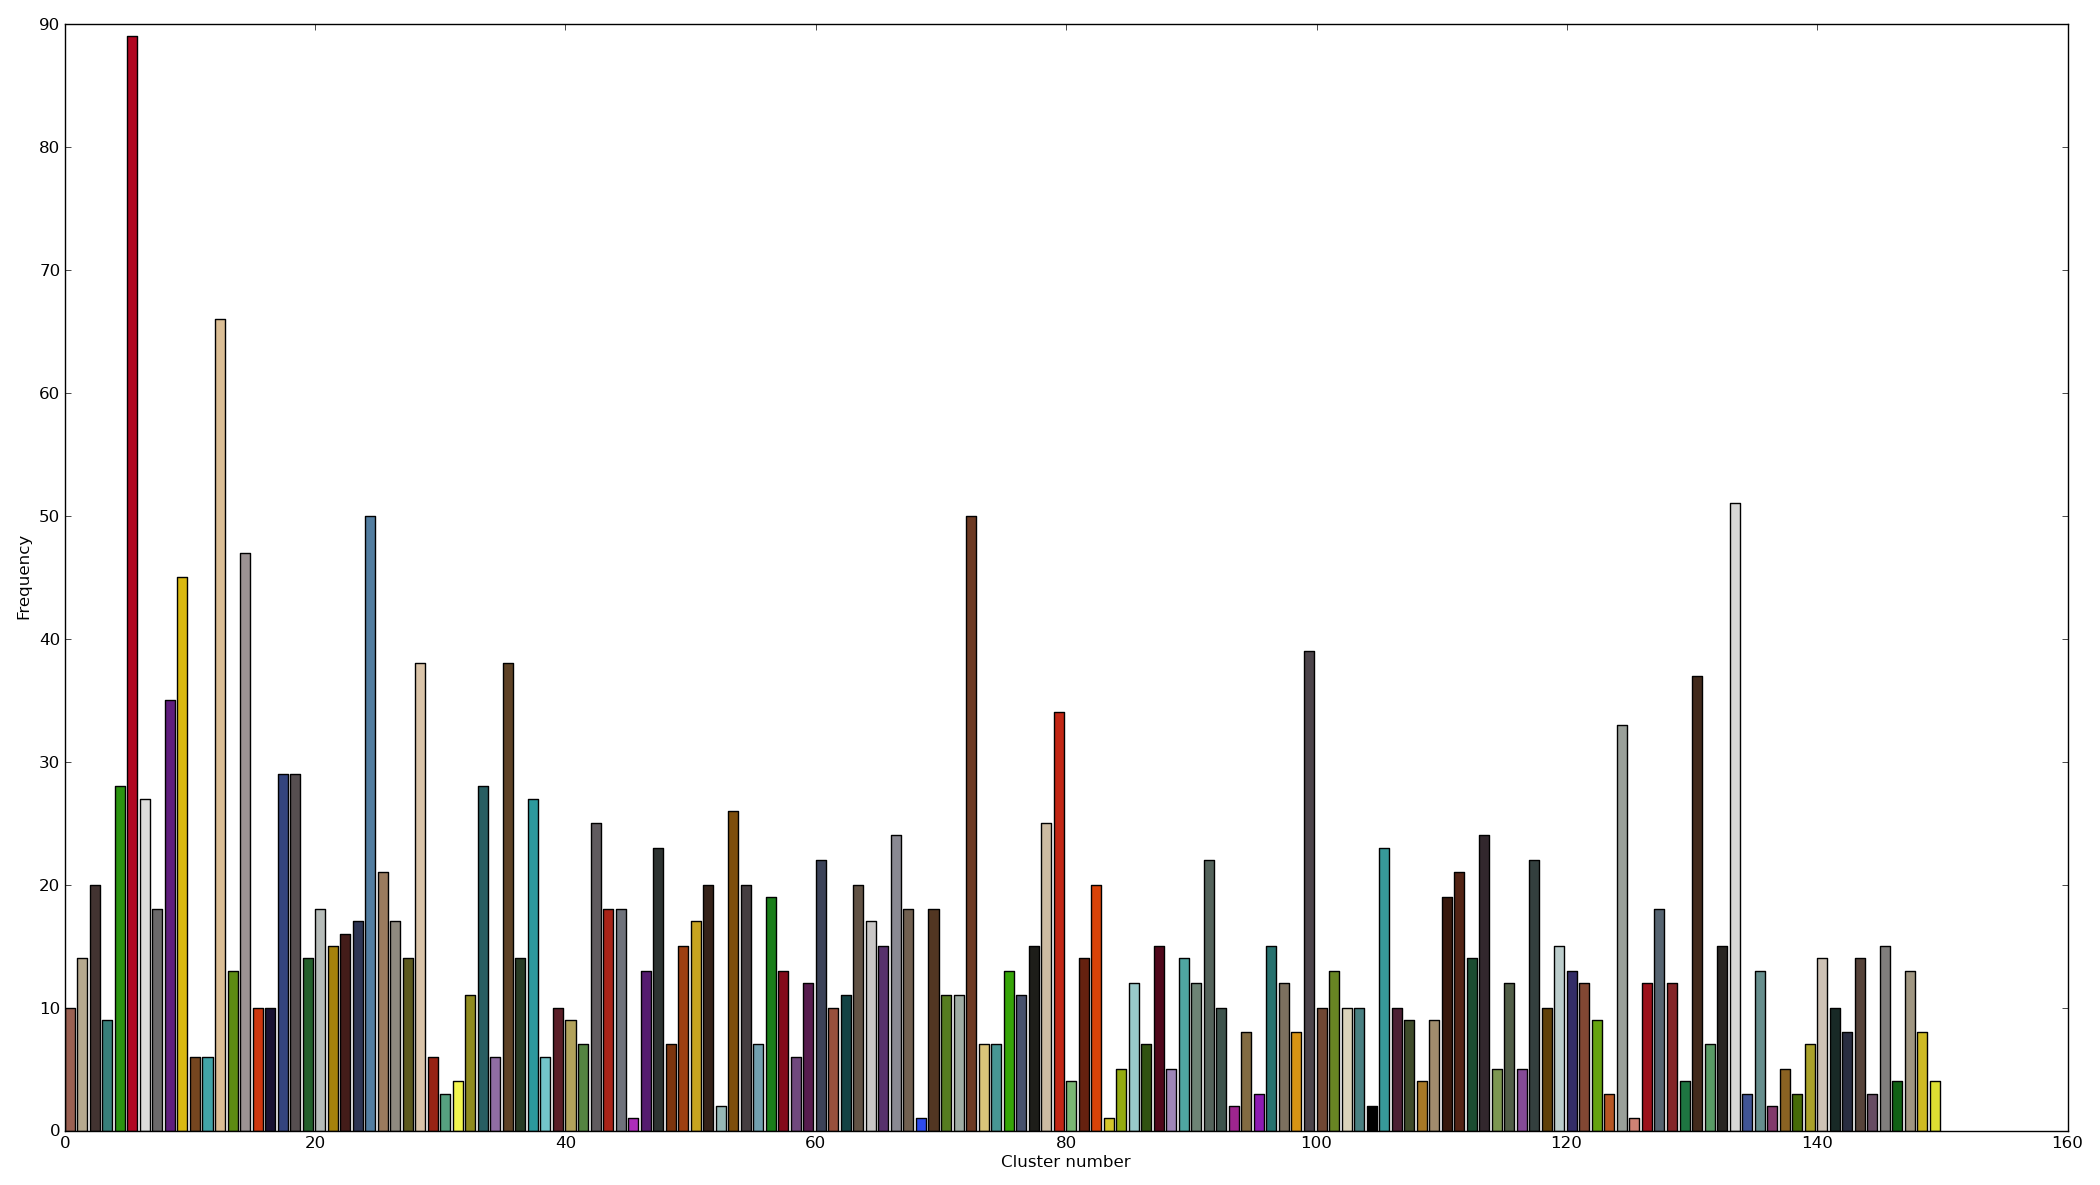
\includegraphics[width=0.90\textwidth]{../150_histogram.png}
  \caption{kmeans histogram with k=150}
  \label{k-150}
\end{figure*}

\begin{figure*}[p]
  \centering
  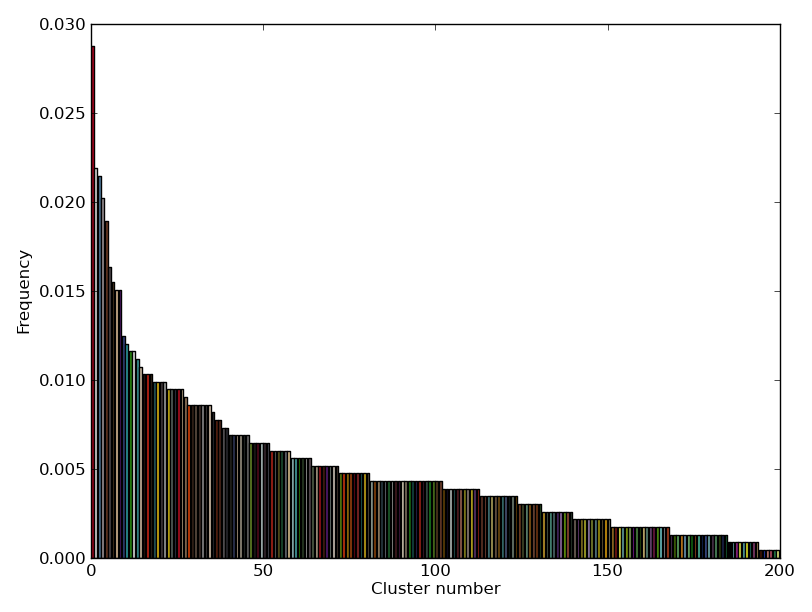
\includegraphics[width=0.90\textwidth]{../200_histogram_sorted.png}
  \caption{kmeans histogram with k=200}
  \label{k-200}
\end{figure*}

\begin{figure*}[p]
  \centering
  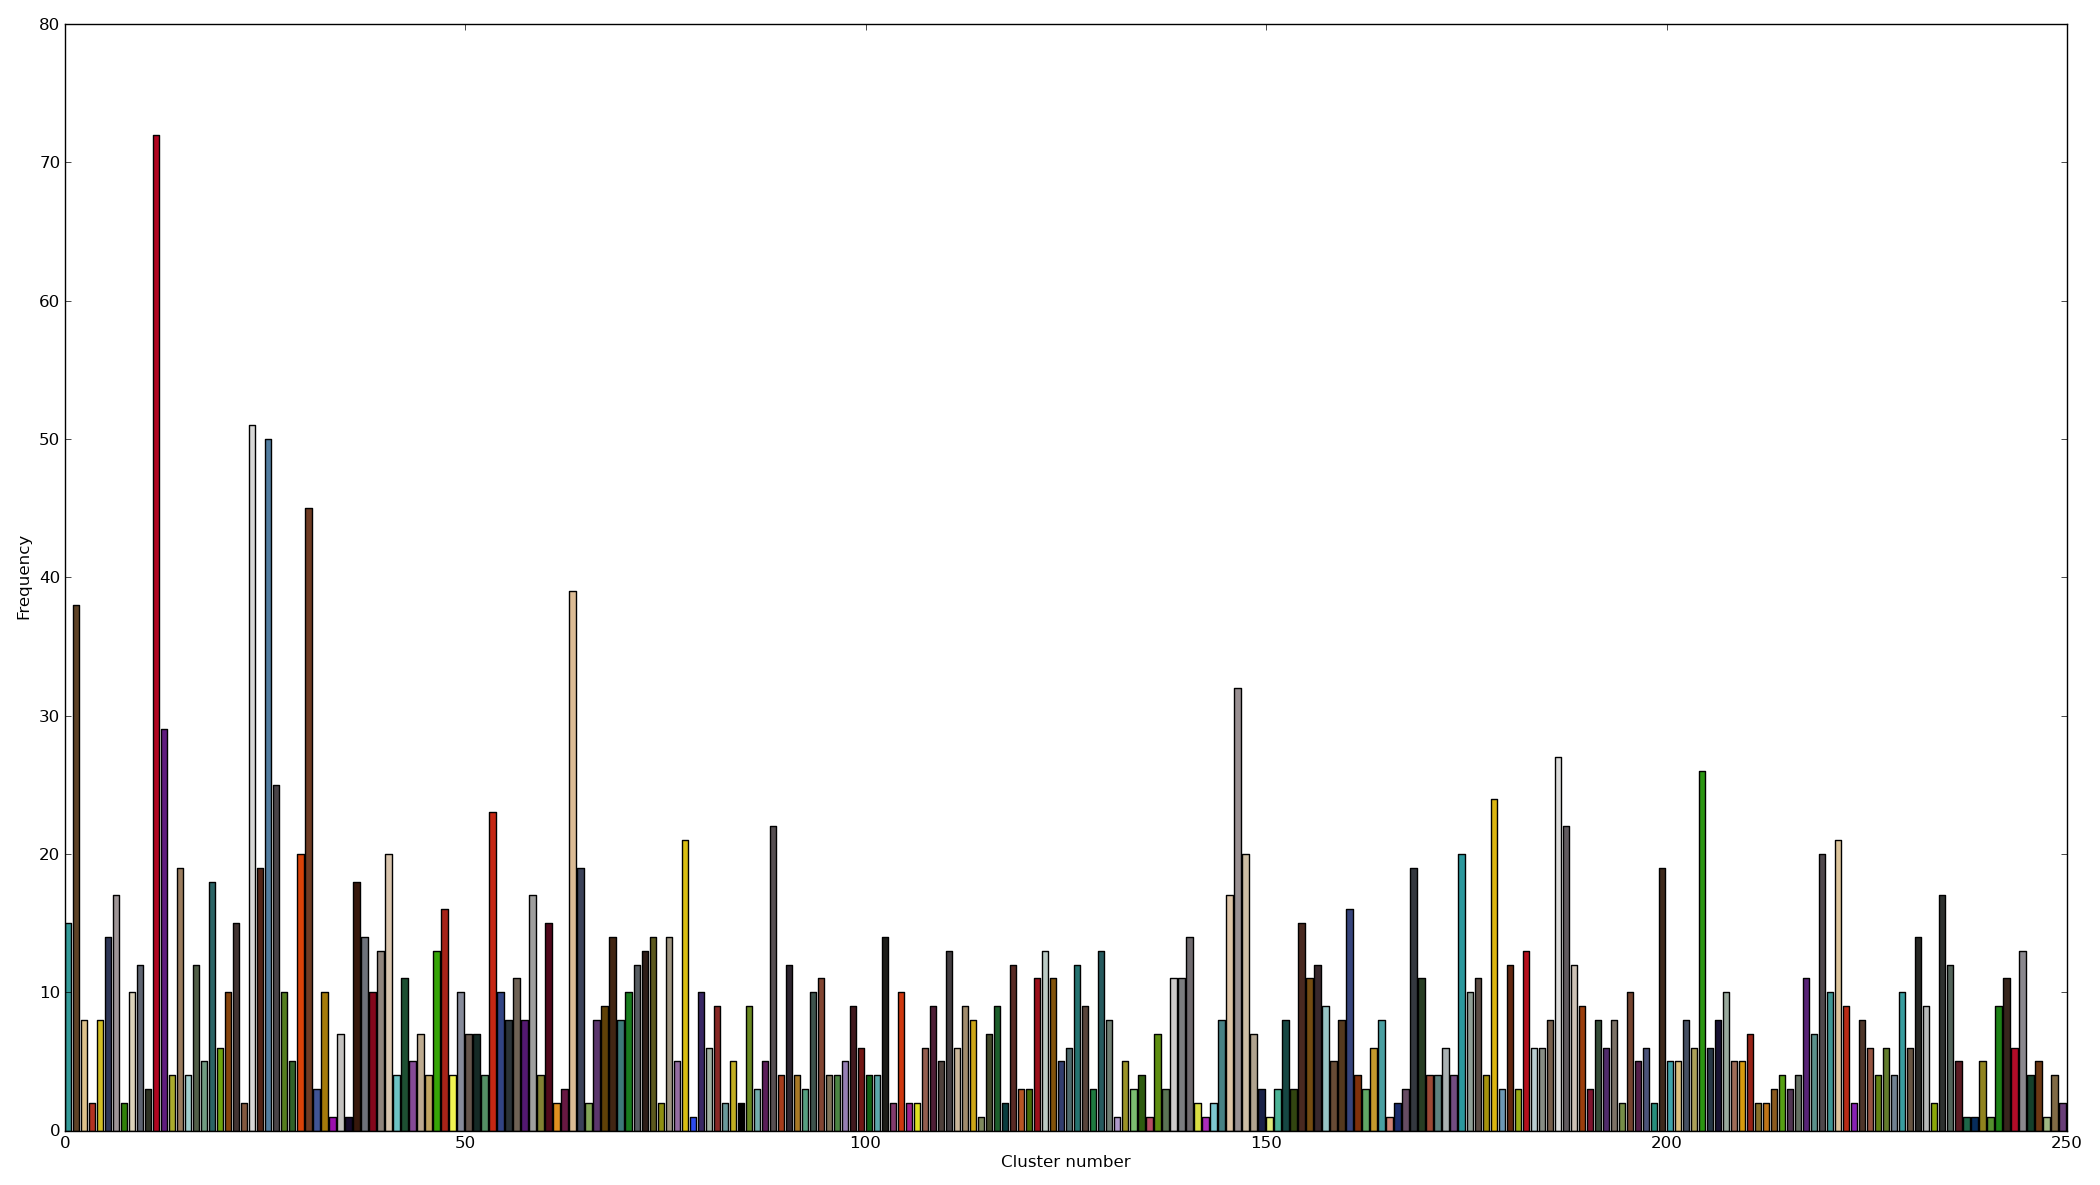
\includegraphics[width=0.90\textwidth]{../250_histogram.png}
  \caption{kmeans histogram with k=250}
  \label{k-250}
\end{figure*}

\begin{figure*}[p]
  \centering
  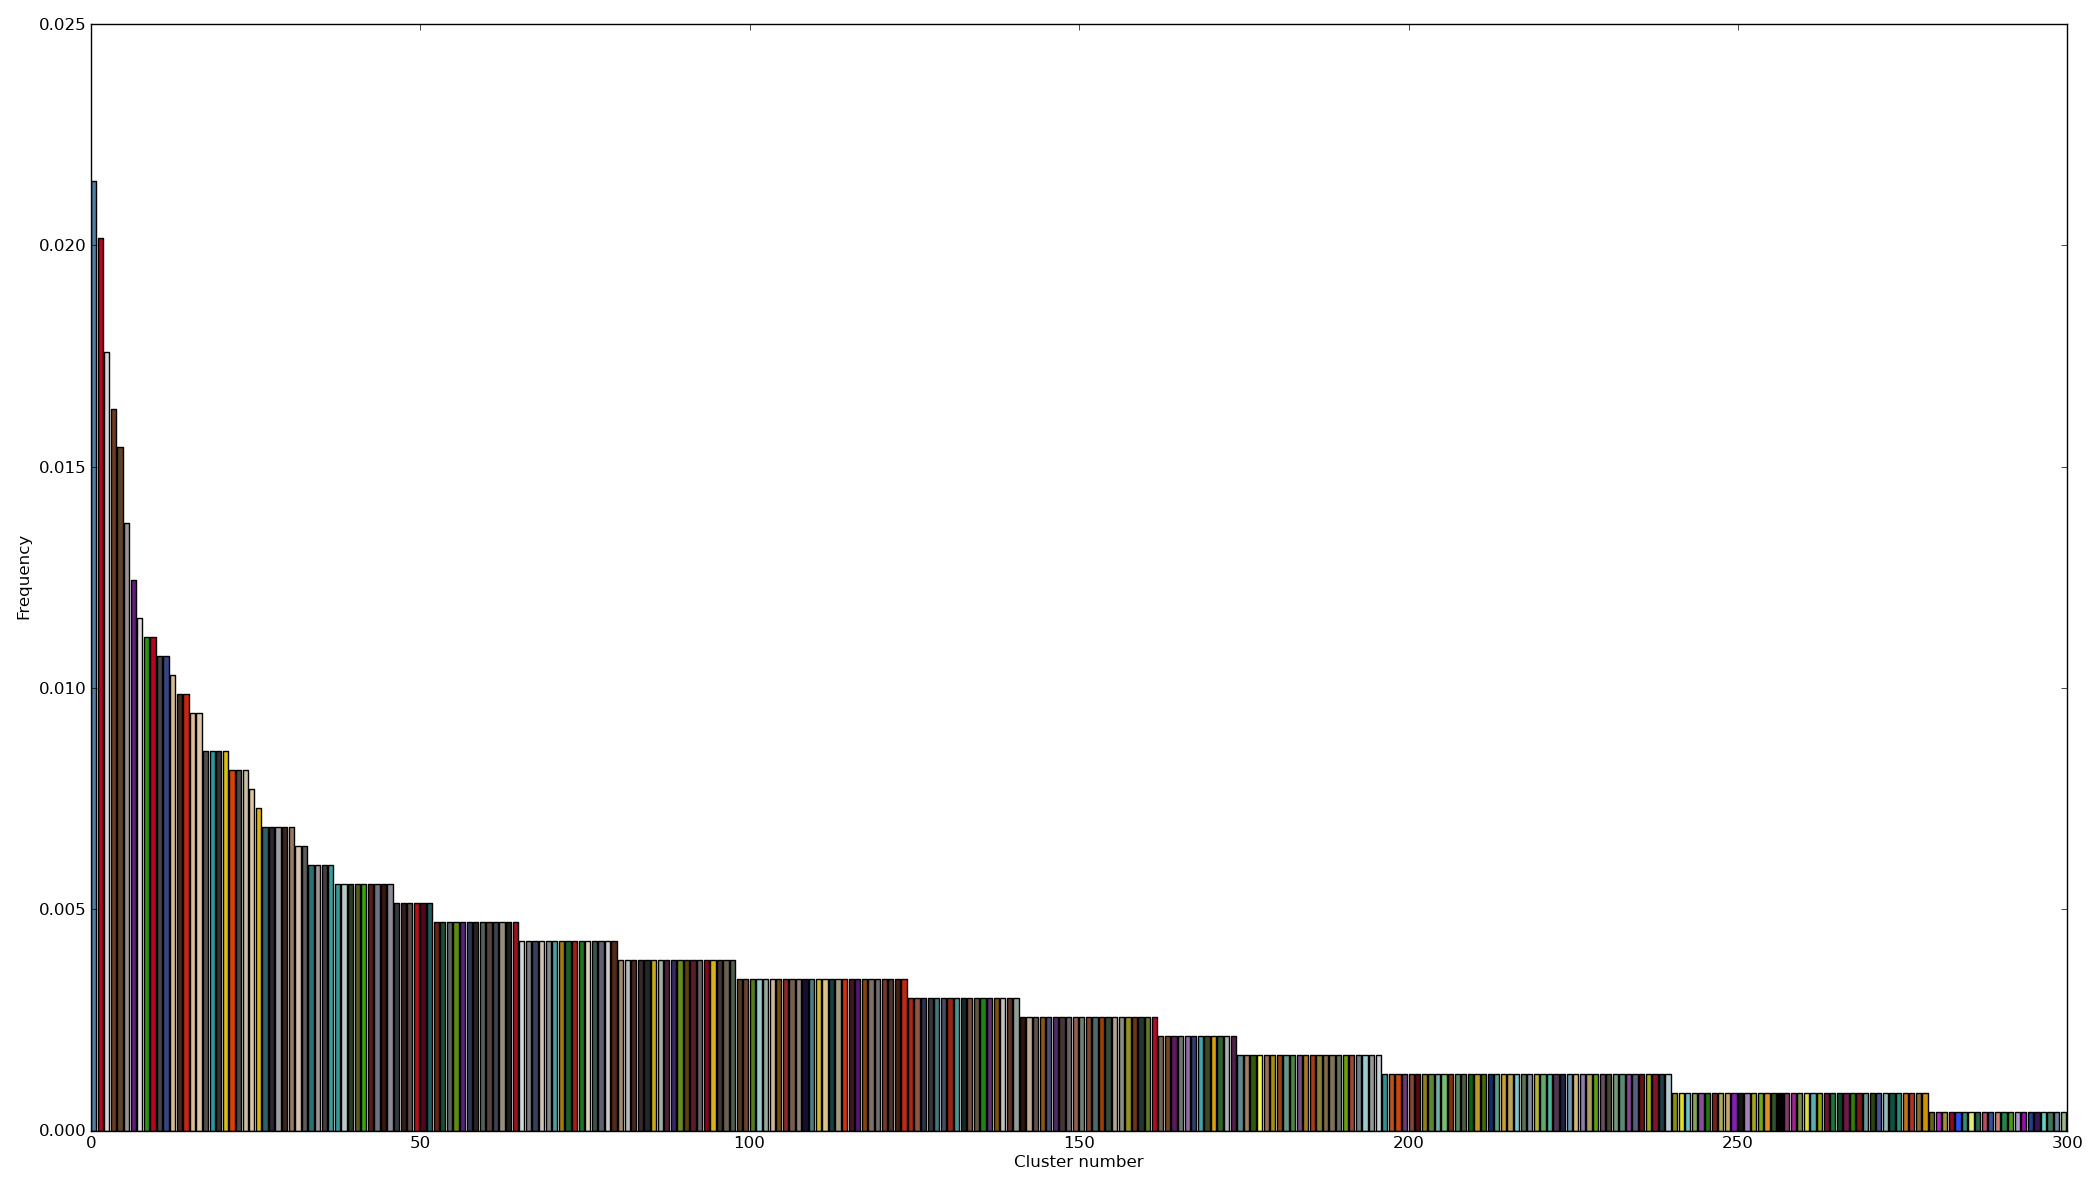
\includegraphics[width=0.90\textwidth]{../300_histogram.png}
  \caption{kmeans histogram with k=300}
  \label{k-300}
\end{figure*}

\begin{figure}[p]
  \centering
  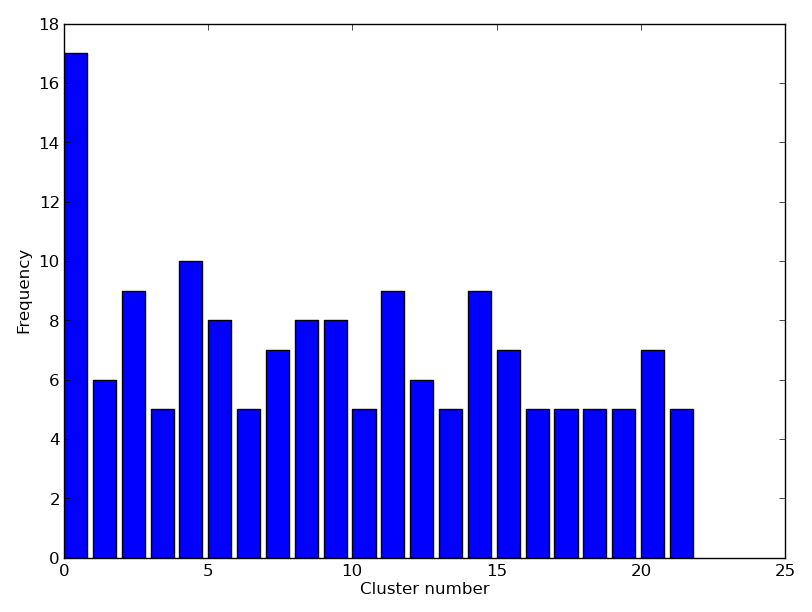
\includegraphics[width=0.50\textwidth]{../dbscan_hist.png}
  \caption{DBSCAN}
  \label{dbscan}
\end{figure}

\begin{figure*}[p] 
  \centering
  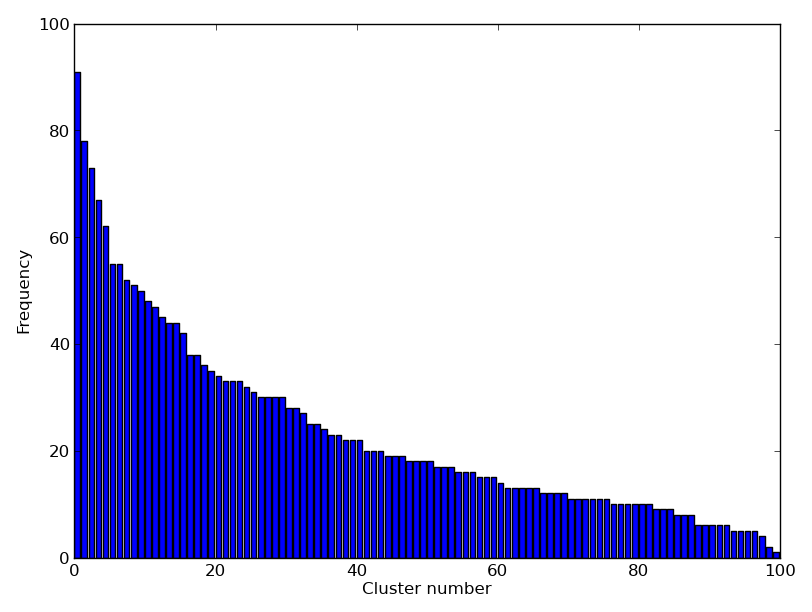
\includegraphics[width=0.90\textwidth]{../agglo_hist.png}
  \caption{Agglomerative clustering with 200 clusters}
  \label{agglo}
\end{figure*}


\subsection{Silhoutte Scores}
\begin{table*}
  \begin{tabular}{|l|l|l||r|r|}
    \hline
    Algorithm & Average(RGB) & Std(RGB) & Average(HSV) & Std(HSV) \\
    \hline
    agglo-200 & 0.458646443848 & 0.269008683093  & 0.465670488369 & 0.260424450724 \\
    agglo-100 & 0.427810049095 & 0.264761260823 & 0.445758372781 & 0.274797481827 \\
    agglo-50 & 0.39460106313 & 0.283348220964 & 0.407061643698 & 0.275471127872 \\
    \hline
    dbscan & -0.59659098259 & 0.459189910187 & Negative Score &   \\
    \hline
    K=400 & 0.484954993451  & 0.269845063645 &  \textbf{0.49477624071} & 0.269644110049 \\

    K=300 & 0.470033927835 & 0.255694124258 & 0.483288003653 & 0.259444221453 \\
    K=250 & 0.468510843432 & 0.254082589179 & 0.465240510022 & 0.261075742016 \\
    K=200 & 0.454357446669 & 0.248596212307 & 0.4609727129 & 0.246014493153 \\
    K=150 & 0.451752086146 & 0.251992960509 & 0.459139455038 & 0.240711074362
 \\
    K=100 & 0.429384756877 & 0.236945657405 & 0.456732628513 & 0.237824162046
\\
    K=50 & 0.415098853996 & 0.233513415301 & 0.430250332809 & 0.223607063326
\\
    \hline
    
  \end{tabular}
  \caption{Averages and standard deviations of the silhoutte scores. HSV colorspace gives a higher score.}
\label{sillyscores}
\end{table*}

\section{Future Work and Conclusion}
Some more clustering algorithms
More robust and usable shape detection
Efficient way to encode neighbour segment information
Multi-episode dictionaries
Application and testing on other animated cartoons
Collection of some ground-truth data by using crowd-sourcing (Amazon
Mechanical Turk etc)

%------------------------------------------------------------------------

\clearpage

{\small
\bibliographystyle{ieee}
\bibliography{egbib}
}

\end{document}
